\documentclass[review]{elsarticle}

\usepackage{changes}

%DRAFT WATERMARK
%\usepackage{draftwatermark}
%\SetWatermarkScale{3}
%END DRAFT WATERMARK

%\usepackage{lineno,hyperref}
%\modulolinenumbers[5]

\usepackage{rotating} % rotate elements in LaTeX
\usepackage{booktabs} % table formatting
\usepackage{wrapfig} % wrapping text around figures
\usepackage{caption} % subfigures
\usepackage{subcaption} % subfigures
\usepackage{makecell} % \thead in tables
\usepackage{amsmath}
\usepackage{amsfonts}
\usepackage{amssymb} % mathematical symbols
\usepackage{bm} % bold mode \bm
\usepackage{multicol}
\usepackage{xcolor}

\usepackage{amsthm} % Theorems
\newtheorem{theorem}{Theorem}%[section]
\newtheorem{corollary}{Corollary}[theorem]
\newtheorem{lemma}[theorem]{Lemma}
\theoremstyle{definition} % definition
\newtheorem{definition}{Definition}%[section]
\newtheorem{proposition}{Proposition}%[section]


\theoremstyle{remark}
\newtheorem*{remark}{Remark}

\newcommand{\me}{\mathrm{e}} % exponential e

\journal{Computer Methods and Programs in Biomedicine}

%%%%%%%%%%%%%%%%%%%%%%%
%% Elsevier bibliography styles
%%%%%%%%%%%%%%%%%%%%%%%
%% To change the style, put a % in front of the second line of the current style and
%% remove the % from the second line of the style you would like to use.
%%%%%%%%%%%%%%%%%%%%%%%

%% Numbered
%\bibliographystyle{model1-num-names}

%% Numbered without titles
%\bibliographystyle{model1a-num-names}

%% Harvard
%\bibliographystyle{model2-names.bst}\biboptions{authoryear}

%% Vancouver numbered
%\usepackage{numcompress}\bibliographystyle{model3-num-names}

%% Vancouver name/year
%\usepackage{numcompress}\bibliographystyle{model4-names}\biboptions{authoryear}

%% APA style
%\bibliographystyle{model5-names}\biboptions{authoryear}

%% AMA style
%\usepackage{numcompress}\bibliographystyle{model6-num-names}

%% `Elsevier LaTeX' style
%\bibliographystyle{elsarticle-num}
%%%%%%%%%%%%%%%%%%%%%%%

\begin{document}

\begin{frontmatter}

\title{Identification and Visualization of the Underlying Independent Causes of the Diagnostic of Diabetic Retinopathy made by a Deep Learning Classifier}
%\tnotetext[mytitlenote]{Fully documented templates are available in the elsarticle package on \href{http://www.ctan.org/tex-archive/macros/latex/contrib/elsarticle}{CTAN}.}

\author[label1]{Jordi de la Torre\corref{cor1}}
\address[label1]{Departament d'Enginyeria Inform\`atica i Matem\`atiques.\\Escola T\`ecnica Superior d'Enginyeria.\\Universitat Rovira i Virgili\\Avinguda Paisos Catalans, 26. E-43007\\
	Tarragona, Spain}
\ead{jordi.delatorre@gmail.com}
\author[label1]{Aida Valls}
\ead{aida.valls@urv.cat}
\author[label1]{Domenec Puig}
\ead{domenec.puig@urv.cat}
\author[label2]{Pedro Romero-Aroca}
\ead{romeropere@gmail.com}


\cortext[cor1]{Corresponding author}



\address[label2]{Ophthalmic Service. University Hospital Sant Joan de Reus\\Institut d’Investigaci\'o Sanit\`aria Pere Virgili (IISPV)\\ Universitat Rovira i Virgili\\Reus (Tarragona)\\Avinguda de la Universitat, 1. E-43204\\Reus, Spain}

\date{Jan 20, 2019}

\begin{abstract}
\emph{Objectives:} Deep learning models are parameterized functions with up to millions of parameters. Such a big parameter set makes impossible a direct interpretation of its internal logic. The goal of this paper is the proposal of a new method for compressing the internal representation of a deep learning classifier, \added{obtaining a smaller set of disentangled feature components, more suitable for human interpretation.}
 
\emph{Methods:} Deep learning models consist of two main parts: a feature extractor and a classifier. The statistical regularities present in the images are mapped by the feature extractor into a lower dimensional representation in the so-called feature space. The classifier combines such features obtaining a final classification. Such internal representations are much smaller than the input space dimensions but are still too big to be interpreted. Furthermore, typically feature dimensions are highly correlated. We propose a method based on the use of an independent component analysis technique for compressing the feature-space. 

\emph{Results:} The method proposed has been used in a deep learning network constructed for the classification of diabetic retinopathy into 5 levels of severity. We find that its initial 64 dimensional internal feature representation can be compressed into a vector of only 3 dimensions, losing only 1.25\% of performance in classification. 

\emph{Conclusions:} \added{This methodology allows the generation of mathematically independent features from the prior linear but highly redundant and correlated internal feature representation. Due to the linear nature of the calculated transformation, the new calculated components can be easily visualized in the input space for scoring pixel importance using any of the existing methods. We present some score maps on eye-fundus images using the pixel-wise explanation model.}

\end{abstract}

\begin{keyword}
deep learning\sep classification\sep compression\sep diabetic retinopathy
\MSC[2010] 68T10
\end{keyword}

\end{frontmatter}

%\linenumbers

\section{Introduction}

Diabetic Retinopathy (DR) is an associated disease derived from diabetes that is caused by the damage of the small blood vessels of the retina. Due to diabetes disease related secondary effects, retinal blood vessels can break down, leak or become blocked; affecting the transport of nutrients and oxygen to parts of the retina, causing impaired vision over time. Early detection allows its treatment and reduces substantially the negatives consequences associated with its development. Eye screening is used by physicians as a way for disease detection. Automatic classifiers can help in disease detection through the increase of the number of preventive analysis done over the diabetic population \cite{pedro2010prevalence}, \cite{romero2011managing}.

Deep Learning (DL) \cite{nature-deep-learning}, \cite{Schmidhuber-nn}, is a subfield of Machine Learning that allow the automatic model construction of very effective image classifiers using a parametric model. These models are able to identify and extract the statistical regularities present in data that are important for optimizing a defined loss function, with the final objective of mapping a high-multidimensional input into a smaller multi-dimensional output (f: $\mathbb{R}^{n} \mapsto \mathbb{R}^{m}, n \gg m$), enabling its categorization is small sets. They are parameterized models that are usually optimized using a stochastic gradient descent algorithm that minimizes a predefined loss function. These models are able to learn the statistical regularities present in data that allow the separation of the predefined classes \cite{Bengio:2013:RLR:2498740.2498889}, \cite{bengio-2009}.

Convolutional neural networks (CNN) are a deep learning subfield that proved to be very effective for image classification, detection and segmentation. The first successful CNN was presented in \cite{LeCun:98}, and it was designed for hand-written digit recognition. This early CNN implementation used a combination of convolution, pooling and non-linearity that has been the key feature of DL since now. The DL breakthrough took place with the publication of \cite{NIPS2012_4824}, where for the first time a CNN won the Imagenet\cite{imagenet_cvpr09} classification competition by a large margin. In that paper a set of innovative techniques where introduced including data augmentation, the use of rectified linear units (ReLUs) as activation function, the use of dropout for avoiding overfitting, overlapping max-pooling for avoiding the averaging effects of avg-pooling and the use of GPUs for speeding up the training time. Later on, different CNN improvements where also published. In \cite{vggnet}, it was the first time that small 3x3 convolution filters where used and combined as a sequence of convolutions. In \cite{he2016deep} the authors introduced residual networks. This networks used a combination of 3x3 convolutional layers with a by-pass of the input every two layers that was summed up to the output. Such bypasses improved the gradient propagation through the network allowing the design of deeper networks and improving the classification capabilities. 
%\vspace{1cm} % just to get a page break. Remove if not required

Ordinal regression is a term used for multi-class classification for the cases where a underlying property can be used for prestablishing an ordering of the classes. Several quality measures exist in the literature of machine learning and statistics for ordinal regression \citep{mehdiyev2016evaluating}. Kappa is a well-known statistic coefficient defined by Cohen \citep{cohen1960coefficient} to measure inter-rater agreement in such cases. Weighted Kappa \citep{cohen1968weighted} is another index used for measuring the goodness of a ordinal regression classification. In this last coefficient, disagreements are penalized proportionally to a power of the distance between classes. The penalization most commonly used is the quadratic. In such cases, the index is commonly referred as Quadratic Weighted Kappa (referred as QWK or $\kappa$ indistinctly in this paper).

In equation \ref{eq:kappa} we show the mathematical definition of QWK.

\begin{equation}
\label{eq:kappa}
\begin{aligned}
&\kappa = 1 - \frac{ \sum_{i,j} \omega_{i,j} O_{i,j} }
{\sum_{i,j} \omega_{i,j} E_{i,j}}\\
\end{aligned}
\end{equation}

, where:
\begin{itemize}
	\item[] $C$: is the number of classes
	\item[] $i, j \in \{ 1, 2, ..., C\}$
	\item[] $O_{i,j}$: the number of observations classified in the i-th category by the prediction model and they are in the j-th category in the correct classification (i.e. "true value").
	\item[] $E_{i,j}$: outer product between the two classification histogram vectors (prediction and "true value"), normalized such that $E$ and $O$ have the same sum.
	\item[] $\omega_{i,j}$: weight penalization for every pair $i,j$. Generally, $\omega_{i,j} = \frac{(i-j)^n}{(C - 1)^n}$. For linear penalization $n = 1$. For quadratic penalization (more commonly used and the studied in this paper): $n = 2$.
\end{itemize}

\added{Examples of the usage of the $\kappa$ index for measuring inter-rater agreement in the medical context are: the measure of reliability in ultrasound scans interpretation \citep{hintz2007interobserver}, the evaluation of expert agreement in diagnosis of glaucoma \citep{varma1992expert}, the evaluation of reliability of radiographic assessment \citep{gunther1999reliability}, the inter-observer agreement evaluation in diabetic retinopathy detection \citep{patra2009interobserver}, among many others.}
	
In this paper we study a technique that allows the \added{compression of the feature space and the identification of the mathematically independent elements of a DR DL classifier. We use a the pixel-wise score propagation method to visualize such independent component (IC) in the input space.} This is done by calculating the minimum number of IC that are able to encode the maximum information about the particular classification. Identifying such components, we minimize the redundancy of feature space and we identify the components that share the minimum mutual information between each other. In that way, under the supposition that the feature extraction phase of the deep learning model has been able to disentangle completely the feature information, we are able to separate the independent elements causing the disease.

\added{The proposed compression method is independent from the visualization method used. For the purpose of this work, we have chosen the visualization method proposed in \cite{de2017deep}, but any other one could be also used for its interpretation.} \added{The novelty of the paper is based on the separation and visualization of the mathematically independent features that expain the DR classification.} We use the assessment of experts clinicians for interpreting such IC.

The paper is structured as follows: in section \ref{sec:related} the current work on DL applied to DR is briefly introduced, then, the main works on interpretation of DL are presented. In section \ref{sec:methods} we present the methods used in the paper, in section \ref{sec:results} we present the results obtained, in section \ref{sec:discussion} we present the discussion showing samples of the kind of visual interpretations given by the proposed model and finally in section \ref{sec:conclusions} we present the final conclusions of our work.

\section{Related Work}\label{sec:related}

DL models have been successfully applied in many medical classification tasks. In \cite{esteva2017dermatologist} a DL classifier was designed achieving dermatologist-level accuracy for skin cancer detection. In \cite{wentao2018deeplung} a 3D CNN for automated pulmonary nodule detection and classification was designed. In \cite{wang2018classification} a CNN Alzheimer's disease classifier with high performance was also described. 

Many DL based DR classifiers have been published in the last years. In \cite{doi:10.1001/jama.2016.17216} a deep learning model was published for the classification of the most severe cases of DR. It was trained using an extended version of the EyePACS dataset, improving the tagging of each image by a voting mechanism between different ophthalmologists for deciding the tag of each image and by increasing the number of images of the original dataset, using in this case about 125,000 graded retina fundus images. This model surpassed the human expert capabilities, reaching at the final operating point approximately  97\% sensitivity and 93.5\% specificity. The main benefit of this model was the high specificity and sensitivity achieved for the prediction of the more severe cases of DR. In \cite{de2017deep} a DL interpretable classifier was published for the prediction of five different disease grades. EyePACS dataset was used for training. The results were close to the obtained by trained ophthalmologists, reaching values of specificity and sensitivity greater than 90\% and excellent inter-rater agreement measured through QWK (QWK=0.844) in the 5 classes disease grading task.

\added{In \cite{raman2018fundus} a review of the different fundus photography based deep learning models for diagnosis of diabetic retinopathy is presented. In \cite{takahashi2017applying} the authors propose a novel AI disease-staging system for grading diabetic retinopathy that involves a retinal area not typically visualized on fundoscopy and another AI that directly suggests treatments and determines prognoses. In \cite{zhou2017deep} the authors propose a multiple instance learning method for DR detection, which jointly learns features and classifiers from data and achieves a significant improvement on detecting DR images and their inside lesions. In \cite{keel2019visualizing} they use an adaptive kernel visualization technique to produce DR image feature maps. Such maps are able to identify lesions causing the disease.}  

\added{Feature compression methods, based on dimensionality reduction techniques, allow the expression of the information present in high dimensional vectors into others that use a lower number of dimensions. Depending on the nature of the transformation applied, they can be classified into: linear methods \cite{cunningham2015linear} and non-linear ones \cite{sarveniazi2014actual}. Typical linear methods include Principal Components Analysis (PCA) \cite{jolliffe2011principal}, Singular Value Decomposition (SVD) \cite{golub1971singular}, Linear Discriminant Analysis (LDA) \cite{mika1999fisher} and Independent Component Analysis (ICA) \cite{hyvarinen2000independent}. Non-linear methods use a non-linear transformation for obtaining the compressed version of the vector space. Typical examples of algorithms of this category are kernel-based versions of the linear ones, like kernel-PCA \cite{mika1999kernel}, kernel-ICA \cite{yang2005kernel}, Multidimensional Scaling (MDS) \cite{borg2003modern}, random projections \cite{fradkin2003experiments}, neural networks derived methods \citep{hinton2006reducing}, t-SNE \cite{maaten2008visualizing} and Uniform Manifold Approximation (UMAP) \cite{DBLP:journals/jossw/McInnesHSG18} between many others.}

\added{Principal Component Analysis (PCA) \cite{jolliffe2011principal} is a linear compression technique that allows the extraction of the most important characteristics from data. The components obtained are sorted by the percentage of the variance explained. This type of transformation allows not only the identification of the number of components required for explaining a predefined percentage of the variance, but also the percentage of variance explained by each one of the individual components.}

Independent Component Analysis (ICA)\cite{hyvarinen2000independent} is a statistical method for the separation of a multi-dimensional random signal into a linear combination of components that are statistically as independent from each other as possible. The theoretical foundation of ICA is based on the Central Limit Theorem, which establishes that the distribution of the sum (average or linear combination) of N independent random variables approaches a gaussian as $N \rightarrow \infty$. When ICA method is applied, it is assumed that such separation exist, ie. that is possible to express the signal as a linear combination of independent components (IC). Perfect independence between random variables is achieved when mutual information between them is zero. Mutual information can be expressed as the Kullback-Leibler divergence between the joint distribution and the product of the distributions of each variable. Mutual information can be decomposed, under linear transforms, as the sum of two terms: one term expressing the decorrelation of the components and one expressing their non-Gaussianity \cite{cardoso2003dependence}. ICA uses optimization to calculate its components. Two types of optimization objectives can be used: minimize the mutual information or maximize the non-gaussianess of each component. 

\added{Being both PCA and ICA linear methods, the difference between them relies in the way the data projection is done. PCA looks for basis vectors that best explain the variance of your data, being orthogonal between each other. ICA sacrifizes orthogonality in favor of minimizing mutual information, ie. maximizing probabililistic independence. In PCA, components are sorted by importance, ie. percentage of variance explained. In ICA, neither the vectors are sorted by order of importance nor it gives information about the percentage of information explained, requiring an external evaluation for fixing the optimal number of components.}

\added{Deep learning models are very successful in the separation of elements in different classes, but they have a major concern, that is the difficulty of interpreting the reasons behind a particular classification. They are parameterized models with not less than tens of thousands of parameters. The interaction between them is very difficult to analyze, making unfeasible a direct interpretation. In last years different ways for result explanation of deep learning models have been developed. In \cite{zeiler2014visualizing} the authors use a propagation method for visualizing the results in pixel-space. In \cite{bach2015pixel} a pixel-wise decomposition is used. The calculated scores are back propagated using a message passing technique allowing the score distribution through all the input pixels. In \cite{zhou2016learning} proposed a technique called Class Activation Mapping (CAM) for identifying discriminative regions used by a restricted class of image classification CNNs which do not contain any fully-connected layers. In \cite{selvaraju2017grad} a generalization of the CAM algorithm was proposed to make it applicable to a significantly broader range of CNN model families without requiring architectural changes or retraining any secondary learning component. In \cite{de2017deep} a pixel-wise derived explanation model was proposed. The model is of general applicability and is able to generate explanations at pixel level, having an expert proved validity for diabetic retinopathy lesion detection being able to infer lesion locations only from the labels of the image classes.} 


\section{Methods}\label{sec:methods}

DL models are organized in layers, being the inputs of each one a combination of the outputs of previous ones. We design the output layer to be a linear combination of last layer feature space components. In this way we are forcing the model to disentangle the important features that, combined in a linear way, allow the achievement of a maximum possible classification score. These components (or other obtained as a linear combination of them, like with ICA analysis), are easy to analyze due to the linear nature of its relationship with the classification scores.

\subsection{ICA based interpretation procedure}

In this paper we go a step forward in the interpretation of score maps. Instead of generating directly the pixel maps associated with a particular class, we try to identify and separate independent elements associated with the disease. Our new contribution comes from the identification, separation and visualization of the IC that explain a particular classification decision. We hypothesize that in order to achieve high performance classification scores, the network has to encode the information required to make the classification. Human experts base its decisions in the number and types of lesions present in the image. That's why in some way, such information has to be present in a disentangled form in last layer feature space, previous to the output layer.  Instead of directly visualizing the more important pixels under a classification decision, we split the information of such last feature layer into independent features using a Independent Component Analysis (ICA). A posteriori we use a pixel-wise relevance propagation derived method to visualize such independent component in input space. In this way, we can, not only generate importance pixel maps, but also differentiate between the underlying independent causes of the disease.

We focus on the last layer feature space, previous to the output layer linear combination, in order to identify its properties and try to isolate the independent elements that are determining the class to which the image is assigned. 
%For this purpose, we use a principal component analysis (PCA)  \cite{pearson1901principal} to appraise the redundancy of this space and a 
We apply ICA \cite{hyvarinen2000independent} using different number of components to identify the minimum of them required to achieve a classification score close enough to the achieved without such a dimensional reduction.  ICA allows to find a linear representation of non-Gaussian data so that the components are statistically independent, or as independent as possible. Such a representation seems to capture the essential structure of the data in many applications, including feature extraction \cite{hyvarinen2000independent}. When the data is not Gaussian, there are higher order statistics beyond variance that are not being taken into account by the PCA technique. While PCA captures only uncorrelated components, these uncorrelated components are not necessarily independent for general distributions. ICA minimizes the mutual information (or relative Kullback-Leibler divergence) of non-Gaussian data because two distributions with zero mutual information are statistically independent \cite{comon1992independent}. 

\added{After the training of the DL model, we apply ICA to the last layer feature space vectors, for calculating the optimal ICA transformational matrix.} Using different number of IC and comparing the classification performance of the original model with the obtained using a linear combination of the reduced number of calculated components, it is possible to find the optimal number of components ($n$) that does not significantly reduce the classification performance of the original model. We modify the original model adding a new layer after the last layer feature space to calculate online the components of every analyzed image. The calculated matrix is embeded in the trained network as a new layer (see fig. \ref{fig:models}). The final classification is achieved linearly combining the low dimensional IC layer. 

\begin{figure}[h!]
	\centering
	\begin{subfigure}[b]{\textwidth}
		\centering
		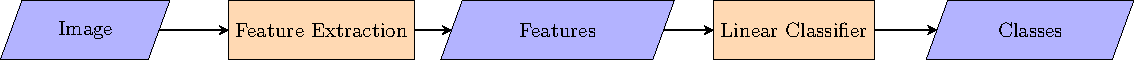
\includegraphics[width=0.7\textwidth]{./figures/initial_classifier.pdf}
		\caption{Initial classification network}	
	\end{subfigure}
	\hfill   
	\begin{subfigure}[b]{\textwidth}
		\centering
		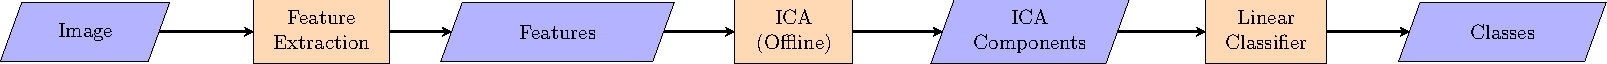
\includegraphics[width=\textwidth]{./figures/ica_classifier.pdf}
		\caption{Modified for feature compression after training}
		\label{fig:models_ica}
	\end{subfigure}
	\caption{Model changes done for compressing feature-space}  
	\label{fig:models} 
\end{figure}

After identifying the optimal $n$, we use the receptive field and pixel-wise explanation model \cite{de2017deep} to visualize the independent scores in the input space. In this way we are visualizing not only a score map explaining a classification but also differentiating and visualizing the mathematically IC responsible of a particular classification. 

\subsection{Mathematical formalization}

Let $F_{train}$ be the set of all feature vectors of training set:

\begin{equation}
	F_{train} = \{\boldsymbol{f^{(i)}} : i = 1 .. T\}, \quad \boldsymbol{f^{(i)}} = (f^{(i)}_1, f^{(i)}_2, ... f^{(i)}_m)
\end{equation}

being $T$ the number of elements of the training set, and $m$ the dimension of feature space vector.

Let $S_{train}$ the set of IC calculated from $F_{train}$:

\begin{equation}
	S_{train} = \{\boldsymbol{s^{(i)}} : i = 1 .. T\}, \quad \boldsymbol{s^{(i)}} = (s^{(i)}_1, s^{(i)}_2, ... s^{(i)}_n)
\end{equation}

being $n$ the number of IC, $n < m$.

Every $\boldsymbol{s^{(i)}}$ can be expressed as a linear combination of $\boldsymbol{f^{(i)}}$:
\begin{equation}
\boldsymbol{s^{(i)}} = \boldsymbol{W} \boldsymbol{f^{(i)}}
\end{equation}

Where $\boldsymbol{W}$ is calculated using a optimization method, minimizing the mutual information between $n$ IC ($\min_{S} I(S)$) \cite{hyvarinen1999fast}.

The ordinal regression problem solved using $F_{train}$ can be expressed as:

\begin{equation}
\max_{\boldsymbol{A}} \big[ \kappa_{val} (C_{train}) \big]
\end{equation}

being:

\begin{equation}
C_{train} = \{ \boldsymbol{A} \boldsymbol{f^{(i)}}, \forall \boldsymbol{f^{(i)}} \in F_{train} \} 
\end{equation}


being $\boldsymbol{c^{(i)}} = \boldsymbol{A} \boldsymbol{f^{(i)}}$ the predicted class vector and $\kappa_{val}$ the evaluation function used in the training process of the neural network calculated for the validation set.

We want to solve the same problem using the reduced ICA components (feature space compressed version):

\begin{equation}
C'_{train} = \{ \boldsymbol{B} \boldsymbol{s^{(i)}}, \forall \boldsymbol{s^{(i)}} \in S_{train} \} 
\end{equation}

being $\boldsymbol{c'^{(i)}} = \boldsymbol{B} \boldsymbol{s^{(i)}}$ the predicted class vector using $n$ IC.

The optimal number of IC to select is the one that minimizes the difference in performance between both models:

\begin{equation}
\min_{n} \big[ \kappa_{val} (C'_{train}) - \kappa_{val} (C_{train}) \big] 
\end{equation}

\subsection{Baseline Model}

\added{We use as base of our study the deep learning model presented in \cite{de2017deep}}. It is a CNN of 17 layers and 391,325 parameters, that expect to receive RGB images of 640x640 pixels of resolution with black background and trimmed borders. Model layers are divided in two groups: the feature extractor and the classifier. The feature extraction has 7 blocks of 2 layers. Every layer is a stack of a 3x3 convolution with stride 1x1 and padding 1x1 followed by a batch normalization and a ReLU activation function. Between every block a 2x2 max-pooling operation of stride 2x2 is applied.  The classifier is a 2x2 convolution. Finally, a 4x4 average-pooling is used for getting a final 64 feature vector that is linearly combined for obtaining the output scores of every class. The feature extractor has 16 filters in the first block, 32 in the second and 64 in all the others.


\section{Results}\label{sec:results}

\subsection{Data}

In this paper we use the EyePACS dataset. For every patient right and left eye images are present. All images are classified by ophthalmologists according to the standard severity scale presented before in \cite{diaclass}. From the $88,650$ images of the dataset, $10,000$ are used for testing purposes, $3,000$ for validation and $75,650$ for training. They are chosen by patient random selection, ie. left and right eye images of each patient must be present in the same set. Due to random selection, class frequency in all sets is expected to be the same. \textcolor{blue}{In table \ref{class:tab:classperc} we show the data distribution of the dataset. It can be observed, that it is an unbalanced dataset that requires sampling techniques for balance it at training time.}

\begin{table}[ht!]
	\centering
	\begin{tabular}{c c c c c } 
		\hline
		 C0 & C1 & C2 & C3 & C4 \\ [0.5ex] 
		\hline\hline
		 73.7\% & 7.0\% & 14.7\% & 2.6\% & 2.0\%\\
		\hline
	\end{tabular}
	\caption[Frequencies of combined occurrence of classes in both eyes]{Frequencies of combined occurrence of classes in both eyes (left: rows, right: columns)}
	\label{class:tab:classperc}
\end{table}

\subsection{Model Modifications}

\added{After training the network,} we calculate the last layer feature space for the whole train set, obtaining a 64-dimensional vector as a representation of each image. \added{We first applied PCA for evaluation of the redundancy of the feature space. We could see that with only 10 components it is possible to explain 99\% of the variance. This fact proves experimentally that the vector components are highly redundant and thus, it is a potentially a highly compressible space.} 

\begin{figure}[h]
	\centering	
	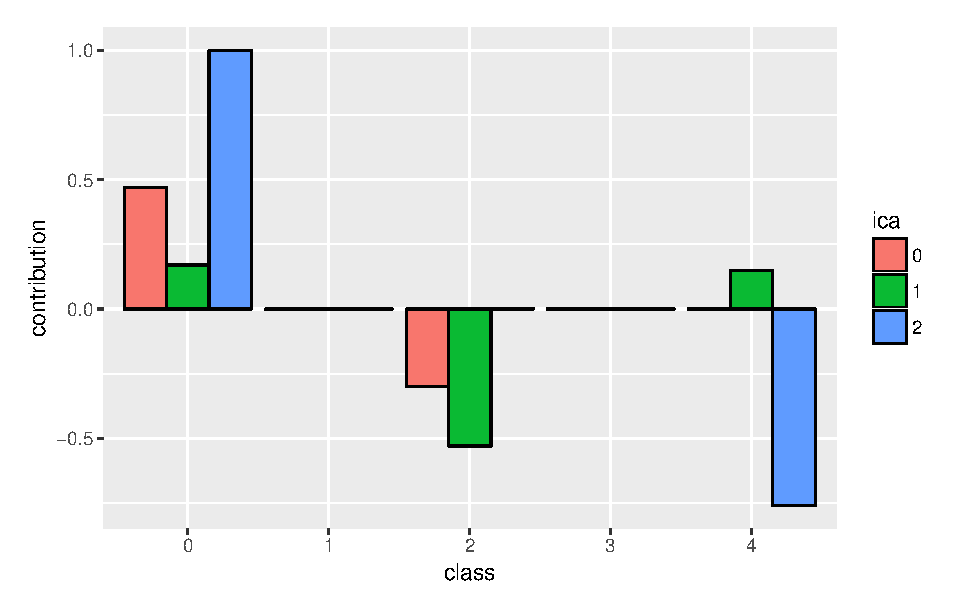
\includegraphics[width=0.90\textwidth]{./figures/ica_class_contribution.eps}
	\caption{Weight of each ICA component in the classification final score (scaling=1e3)}
	\label{fig:ica_contribution}
\end{figure}

After this experiment, our goal was to find a set of ICAs using the 64-dimensional feature-space vectors ($m=64$) of the training set. As we do not know the best number of ICAs, different values of $n$ are explored. With each one, we train a linear classifier to calculate the evaluation metric obtained over a validation set (fig. \ref{fig:models_ica}). We choose the minimal $n$ that allows achieving maximum performance. The optimal $n$ for this problem is $3$, achieving a $QWK_{val} = 0.790 \pm 0.01$ (95\% confidence) not far from the achieved by the original model without dimensionality reduction ($QWK_{val} = 0.800 \pm 0.01$ (95\% confidence)). 

Figure \ref{tab:cm_orig} shows the original confusion matrix. Figure \ref{tab:cm_ica} the confusion matrix after applying ICA. We calculate sensitivity (SN), specificity (SP) and $F_1$ score for Classes 0, 1 vs Classes 2,3,4 for the original model and for the derived ICA model. The values for the original model, acording to its confusion matrix are SN=0.930, SP=0.894, $F_1$=0.776. The values for the ICA derived model are SN=0.950, SP=0.800 and $F_1$=0.796
\begin{figure}
	\centering
	\begin{tabular}{l|lllll}
		& T0 & T1 & T2 & T3 & T4 \\
		\hline
		P0 & 6584 &  673 &  74 &  11 &  21 \\
		P1 & 316 &  367 &  45 &   1 &   2 \\
		P2 & 206 &  366 & 539 & 320 &  30 \\
		P3 & 8 &    6 &  48 & 146 &  12 \\
		P4 & 5 &    8 &  14 &  42 & 156 \\
	\end{tabular}
	\caption{Test set confusion matrix of original model (T: tagged, P: predicted)}
	\label{tab:cm_orig}	
\end{figure}

Fig. \ref{fig:ica_contribution} shows the contribution of each component to the score of each class. We can see that ICA values distinguish clearly three classes (0, 2 and 4) but not class 1 and class 3. The same can be observed in the ICA confusion matrix.

\added{In this regard, it is important to note that Diabetic retinopathy is an ordinal regression problem, where classes 1 and 3 are defined as intermediate transitions between the other classes. Thus, we can see that this automatic model maintains the quality of prediction in terms of the QWK index by just using the 3 most relevant classes, despite doctors are normally using the 5 categories.} 


\begin{figure}
	\centering
	\begin{tabular}{l|lllll}
		& T0 & T1 & T2 & T3 & T4 \\
		\hline
		P0 & 7152 &  505 &  370 &  9 &  10 \\
		P1 & 0 &  0 &  0 &   0 &   0 \\
		P2 & 168 &  223 & 837 & 71 &  18 \\
		P3 & 0 &    0 &  0 & 0 &  0 \\
		P4 & 10 &   3 &  267 &  160 & 197 \\
	\end{tabular}
	\caption{Test set confusion matrix of the ica derived model (T: tagged, P: predicted)}
	\label{tab:cm_ica}	
\end{figure}


As we are training the network using as a loss function $QWK$, the optimization takes place as an ordinal regression. We expect the network to find the underlying causes present in the image that produce the predefined sorting of the classes, ie. the types of lesions and the number of them. Class 0 score contributions come from $ICA_0 > 0$, $ICA_1 > 0$ and $ICA_2 > 0$; being the class markers of the presence of disease $ICA_0 < 0$, $ICA_1 < 0$ and $ICA_2 < 0$.

We use a two-dimensional t-SNE visualization \cite{maaten2008visualizing} for qualitative evaluation of the difference between the quality of the separation using the 64 feature vector and the reduced version with only 3 ICA components. In fig. \ref{fig:tsne} we show the 2D t-SNE visualization for the original feature space and for the ICA reduced space. We can see how for both spaces class 0, 2 and 4 classes are clearly separated. Class 0 and 1 are not properly separated and in the case of 3 and 4, although the separation is not perfect, it is possible to distinguish a different location of both classes for both spaces. 

\begin{figure}[h]
	\centering
	\begin{subfigure}[b]{0.49\textwidth}
		\centering
		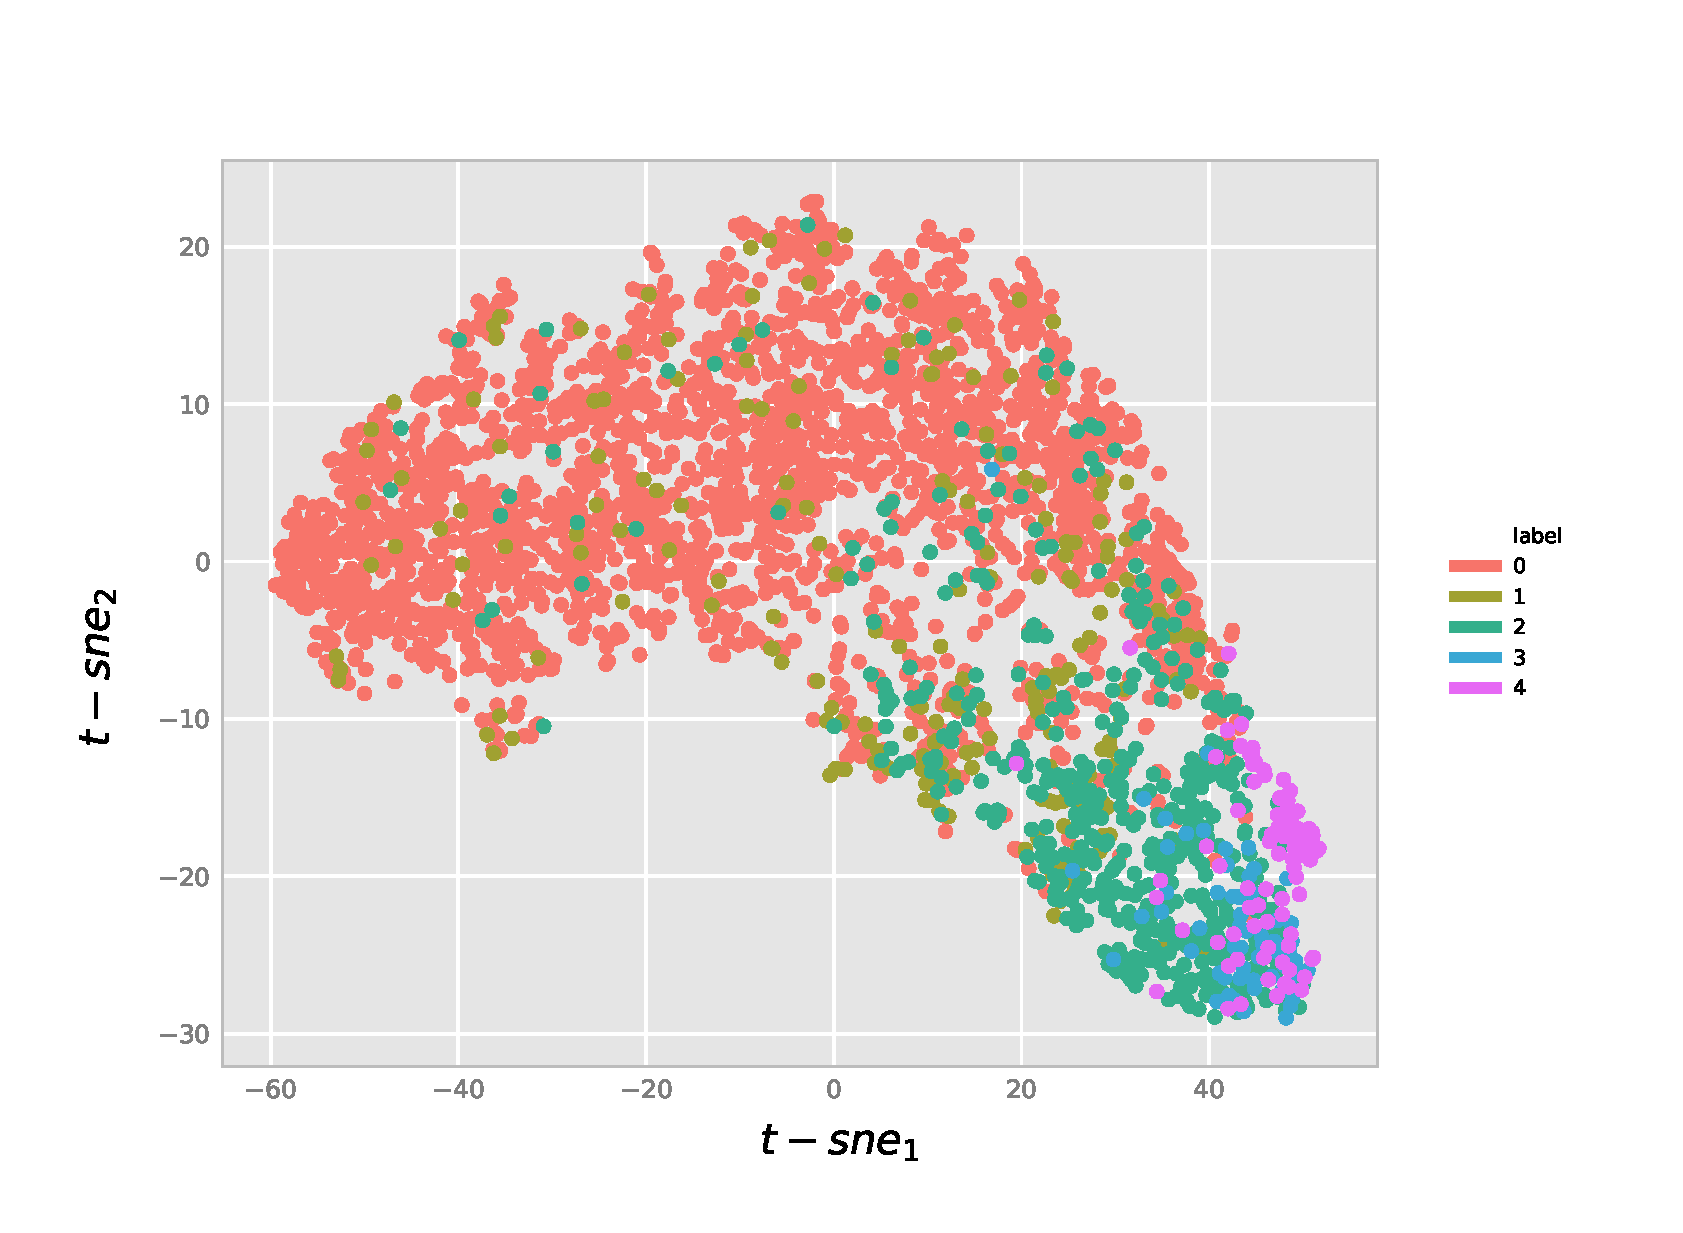
\includegraphics[width=\textwidth]{./figures/tsne2d_p75.eps}
		\caption{Original feature space (64 components)}	
	\end{subfigure}
	\begin{subfigure}[b]{0.49\textwidth}
		\centering
		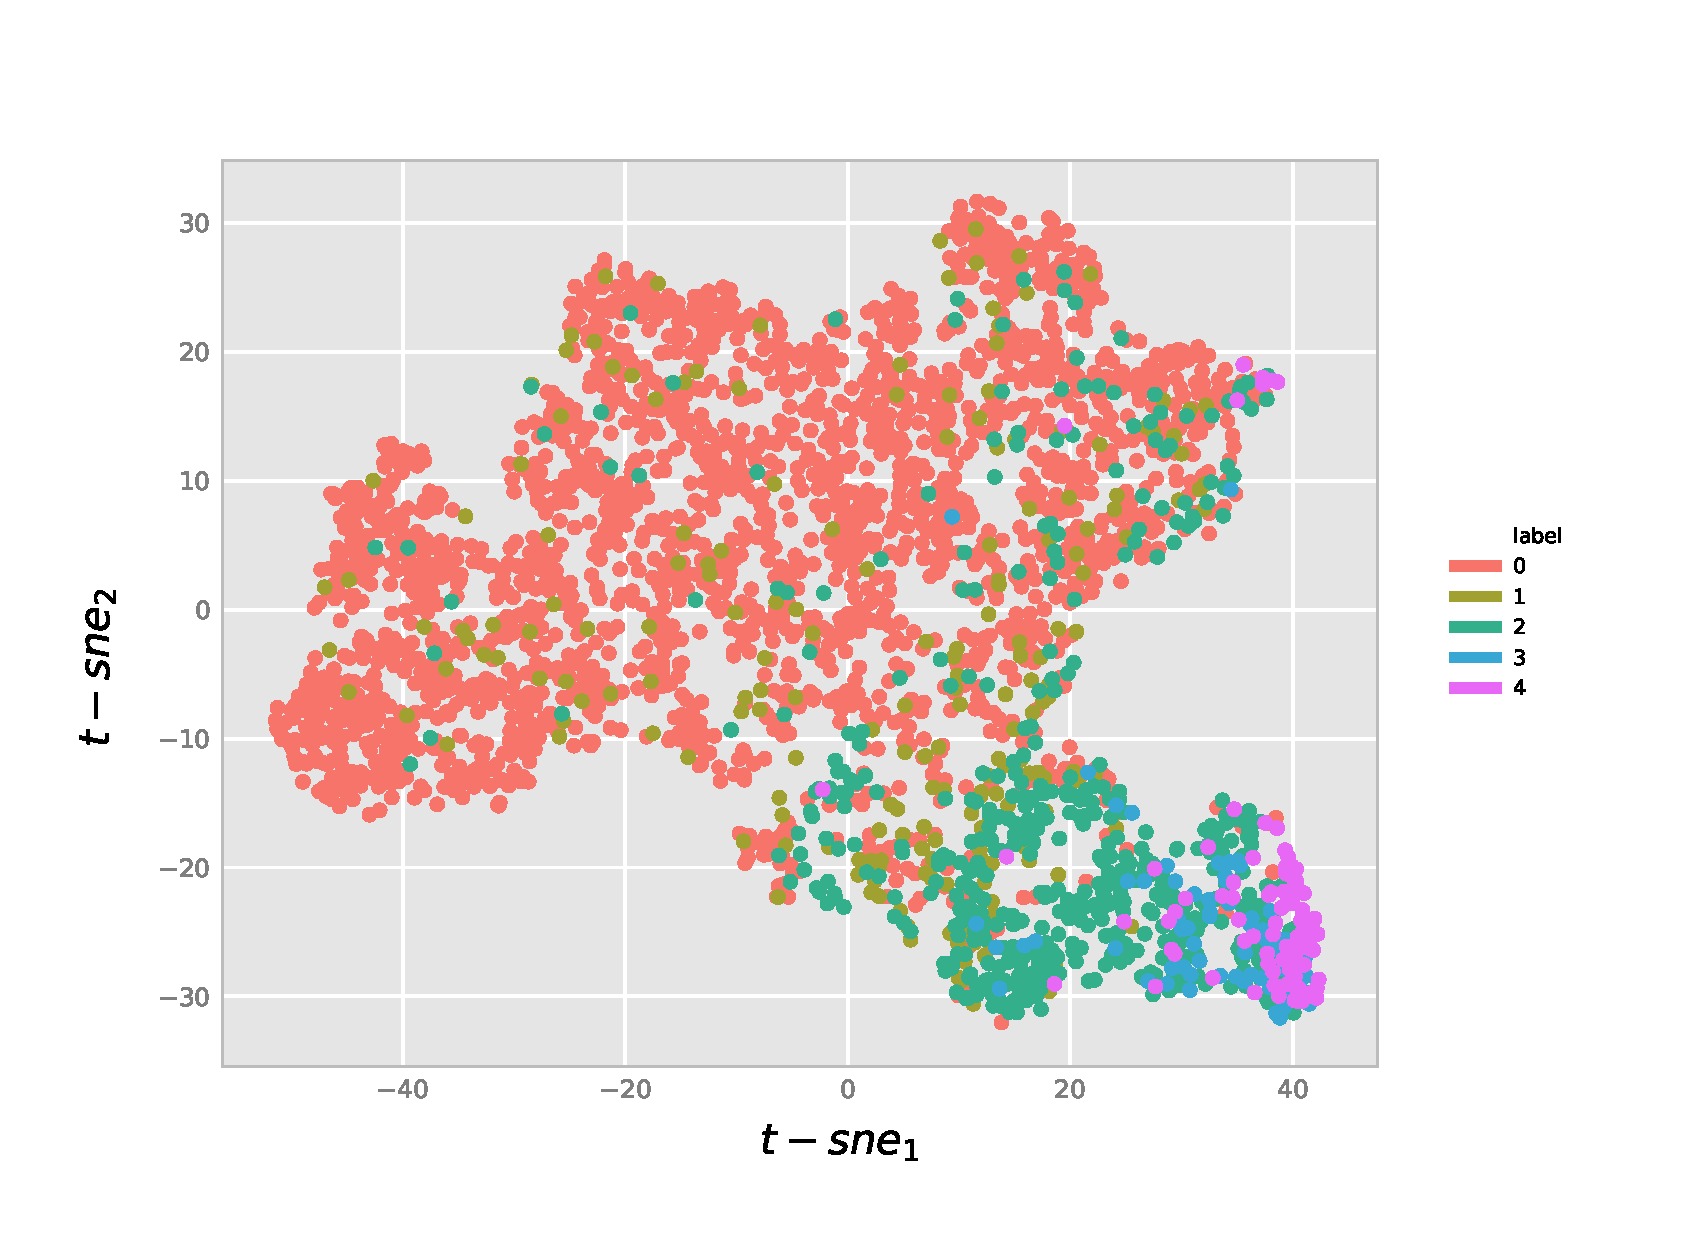
\includegraphics[width=\textwidth]{./figures/tsne2d_ica_p75.eps}
		\caption{ICA space (3 components)}
	\end{subfigure}
	
	\caption{Comparison between the 2D t-SNE visualization of validation set using the original feature space and the final 3-dimensional ICA space}  
	\label{fig:tsne} 
\end{figure}

\subsection{Score components contribution for different test samples}

We apply a pixel-wise relevance propagation method to visualize each ICA component independently. In this way, it is possible to visualize the mathematically independent contributions of each axis and finding the localization of different types of primary elements causing the disease. 

\added{Figures \ref{fig:ica_components_class1}, \ref{fig:ica_components_class2} and \ref{fig:ica_components_class4} show the intermediate score maps generated using a receptive field of 61x61. Figures \ref{fig:ica_components_class1_from}, \ref{fig:ica_components_class2_from} and \ref{fig:ica_components_class4_from} show the original retinographies and the most important lesion zones identified by expert ophtalmologists prior to the generation of ICA lesion maps.}

\begin{figure}[h!]
	\centering
	\begin{subfigure}[b]{0.28\textwidth}
		\centering
		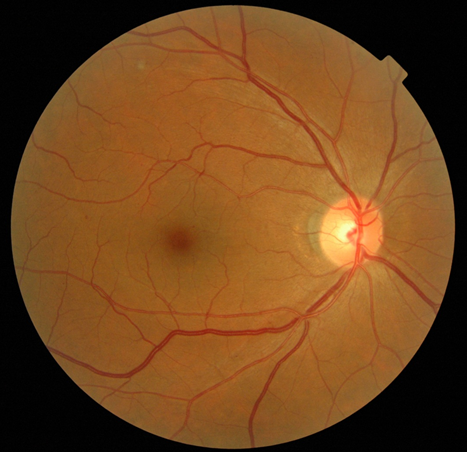
\includegraphics[width=\textwidth]{./figures/ica_retine_maps/G1-P2/g1.png}
		\caption{Original image}	
	\end{subfigure}
	\begin{subfigure}[b]{0.28\textwidth}
		\centering
		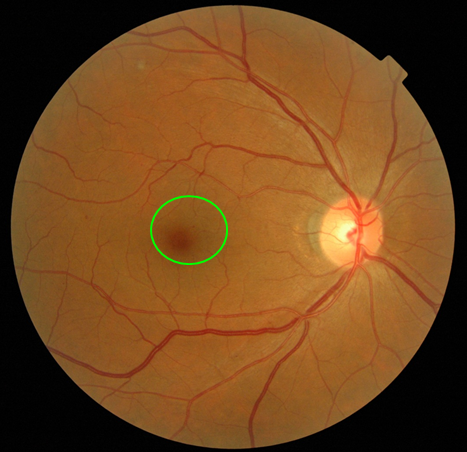
\includegraphics[width=\textwidth]{./figures/ica_retine_maps/G1-P2/metge.png}
		\caption{Real lesion zones}	
	\end{subfigure}
	\hfill 
	\caption{Class 1 image}  
	\label{fig:ica_components_class1_from} 
\end{figure}


\begin{figure}[h!]
	\centering
	\begin{subfigure}[b]{0.32\textwidth}
		\centering
		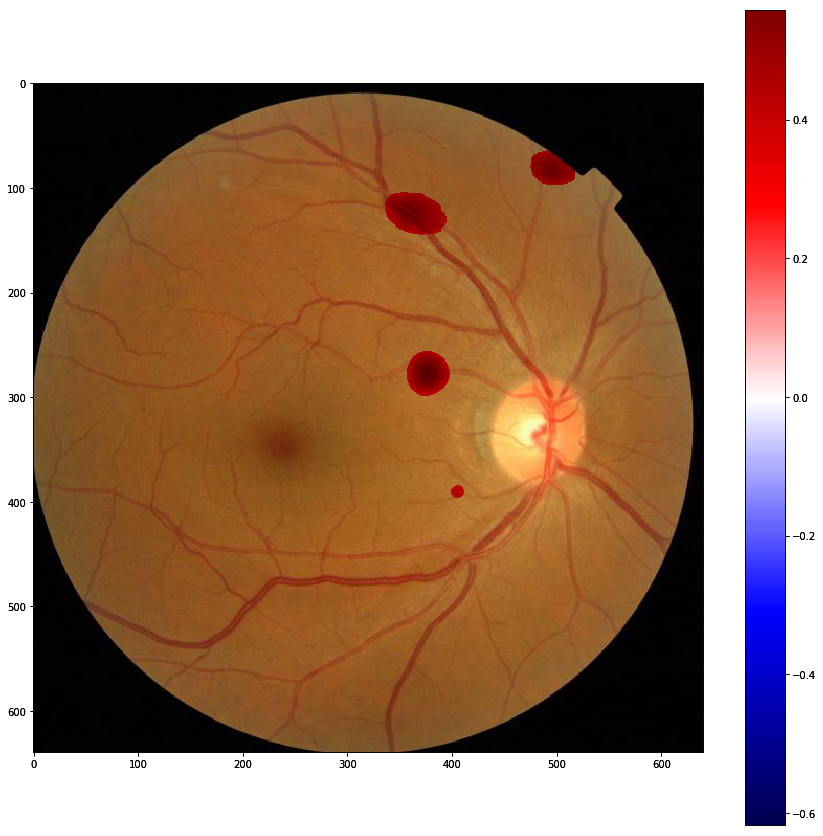
\includegraphics[width=\textwidth]{./figures/ica_retine_maps/G1-P2/m00.png}
		\caption{$ICA_0 < - 3 \sigma$}	
	\end{subfigure}
	\begin{subfigure}[b]{0.32\textwidth}
		\centering
		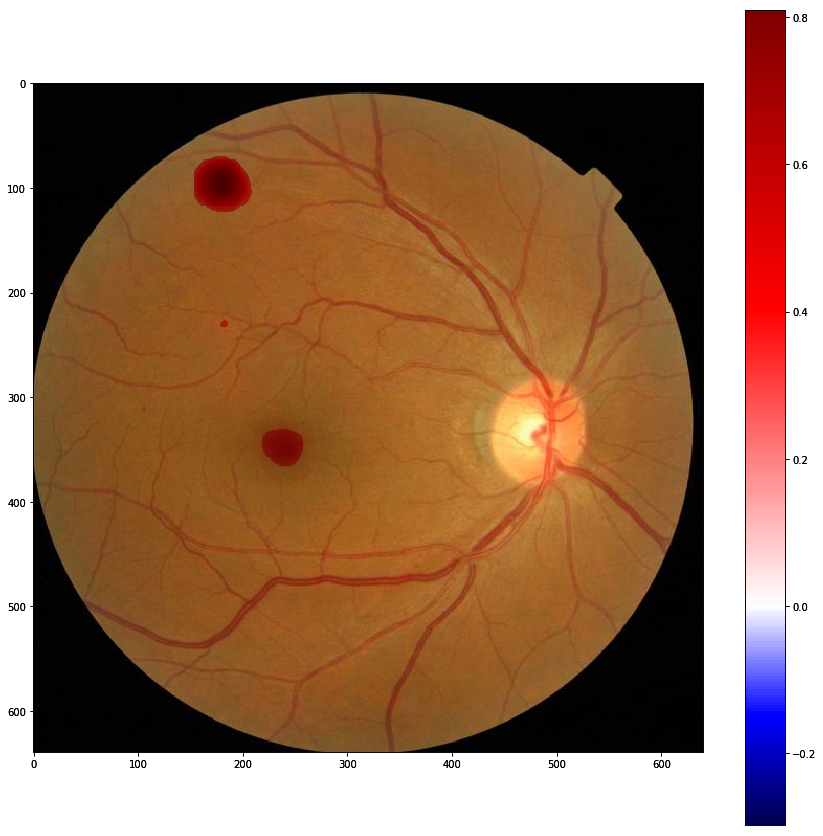
\includegraphics[width=\textwidth]{./figures/ica_retine_maps/G1-P2/m01.png}
		\caption{$ICA_1 < - 3 \sigma$}	
	\end{subfigure}
	\begin{subfigure}[b]{0.32\textwidth}
		\centering
		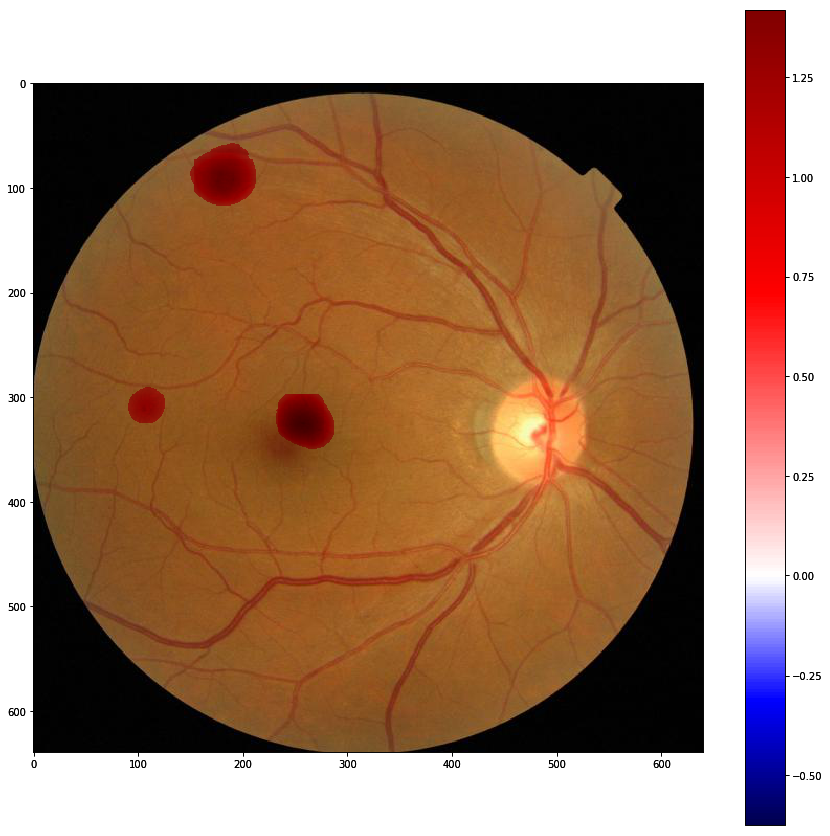
\includegraphics[width=\textwidth]{./figures/ica_retine_maps/G1-P2/m02.png}
		\caption{$ICA_2 < - 3 \sigma$}	
	\end{subfigure}
	\hfill 
	\caption{ICA explanation maps generated using a receptive field of 61x61}  
	\label{fig:ica_components_class1} 
\end{figure}

\added{Figure \ref{ica_components_class1_from} show an example of a mild case of DR. We present the results obtained from the model to an expert ophtalmologist in order to validate the results. The expert concludes that all the regions identified by $ICA_1$ and $ICA_2$ correspond to real lesions. In the case of $ICA_0$ the expert identifies the top center zone as a false positive.}


\begin{figure}[h!]
	\centering
	\begin{subfigure}[b]{0.28\textwidth}
		\centering
		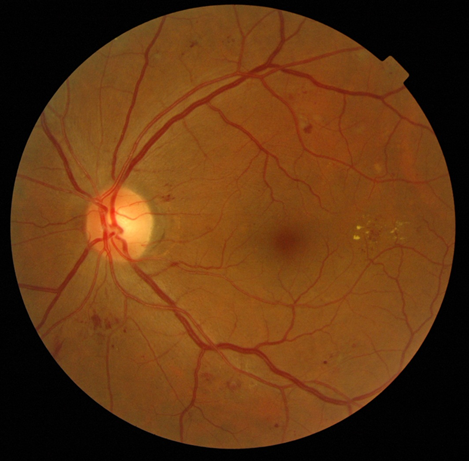
\includegraphics[width=\textwidth]{./figures/ica_retine_maps/G2-P3/g2.png}
		\caption{Original image}	
	\end{subfigure}
	\begin{subfigure}[b]{0.28\textwidth}
		\centering
		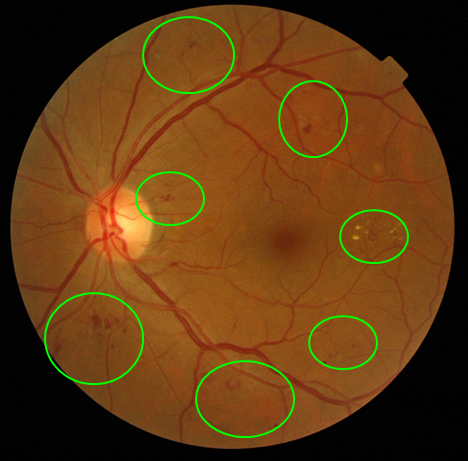
\includegraphics[width=\textwidth]{./figures/ica_retine_maps/G2-P3/metge.png}
		\caption{Real lesion zones}	
	\end{subfigure}
	\hfill 
	\caption{Class 2 image}  
	\label{fig:ica_components_class2_from} 
\end{figure}


\begin{figure}[h!]
	\centering
	\begin{subfigure}[b]{0.32\textwidth}
		\centering
		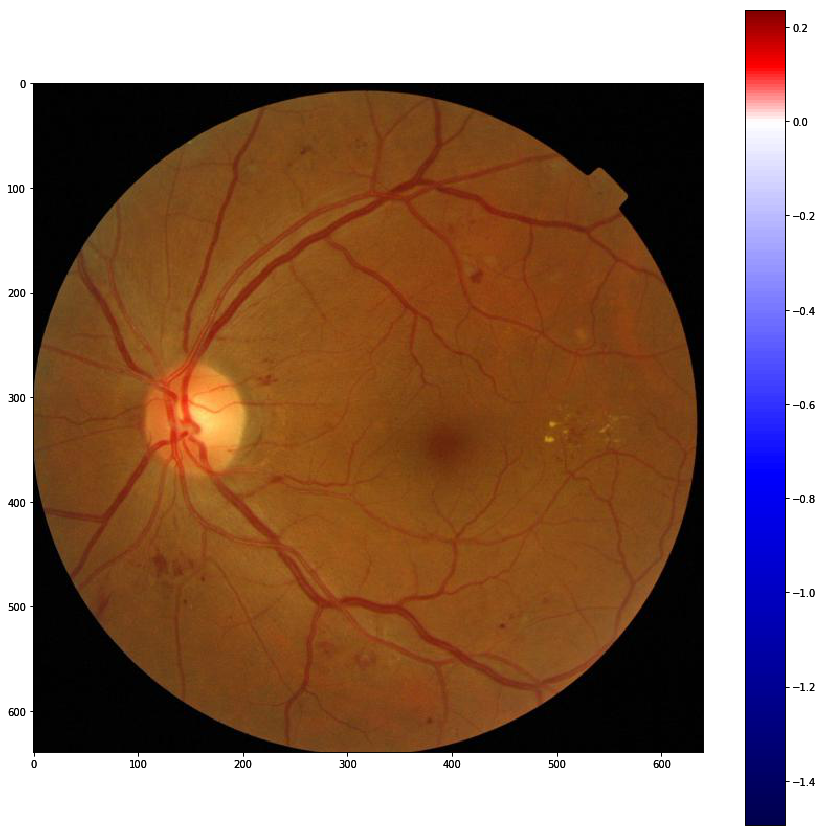
\includegraphics[width=\textwidth]{./figures/ica_retine_maps/G2-P3/m10.png}
		\caption{$ICA_0 < - 3 \sigma$}	
	\end{subfigure}
	\begin{subfigure}[b]{0.32\textwidth}
		\centering
		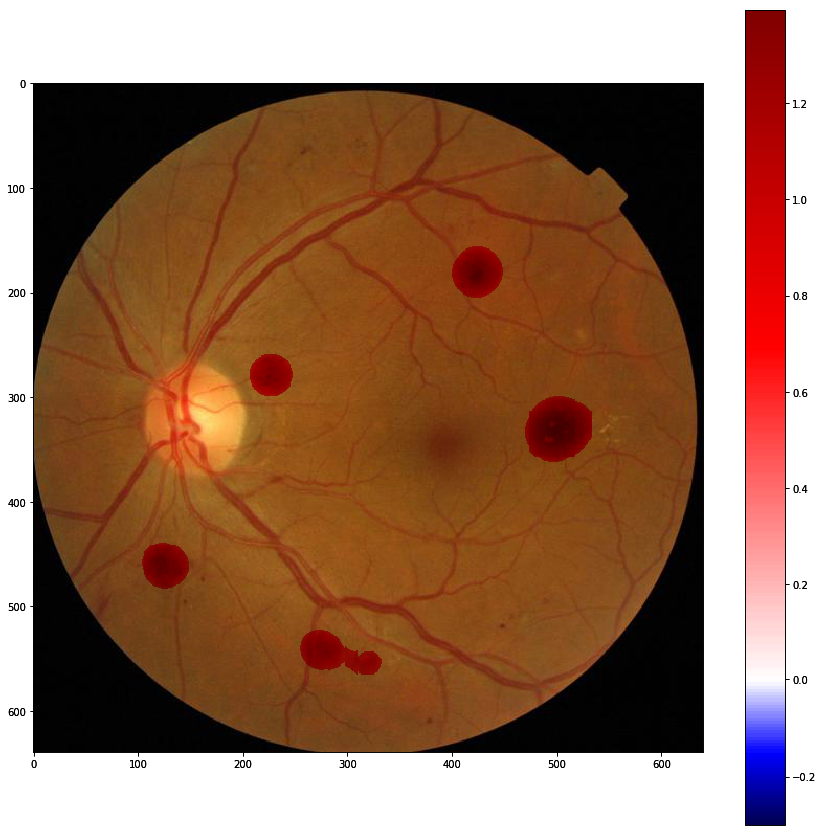
\includegraphics[width=\textwidth]{./figures/ica_retine_maps/G2-P3/m11.png}
		\caption{$ICA_1 < - 3 \sigma$}	
	\end{subfigure}
	\begin{subfigure}[b]{0.32\textwidth}
		\centering
		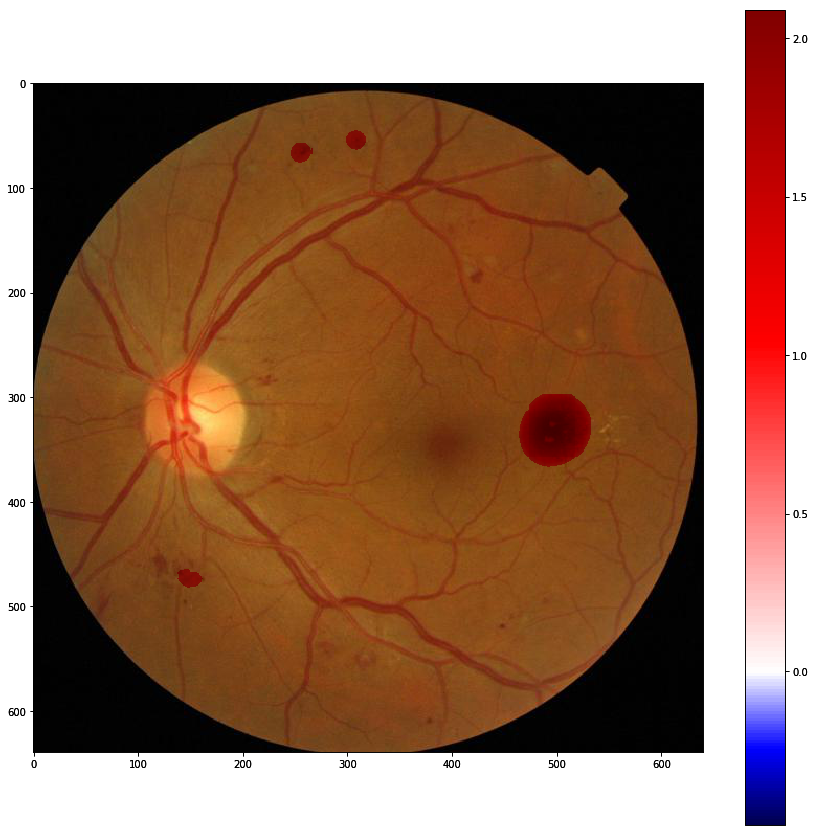
\includegraphics[width=\textwidth]{./figures/ica_retine_maps/G2-P3/m12.png}
		\caption{$ICA_2 < - 3 \sigma$}	
	\end{subfigure}
	\hfill 
	\caption{ICA explanation maps generated using a receptive field of 61x61}  
	\label{fig:ica_components_class2} 
\end{figure}

\added{Figure \ref{ica_components_class2_from} show an example of a moderate case of DR. We present the results obtained from the model to an expert ophtalmologist in order to validate the results. The expert concludes that all the regions identified by $ICA_1$ and $ICA_2$ correspond to real lesions. In the case of $ICA_0$ in this case, no lesion zones are detected by the model.}

\begin{figure}[h!]
	\centering
	\begin{subfigure}[b]{0.28\textwidth}
		\centering
		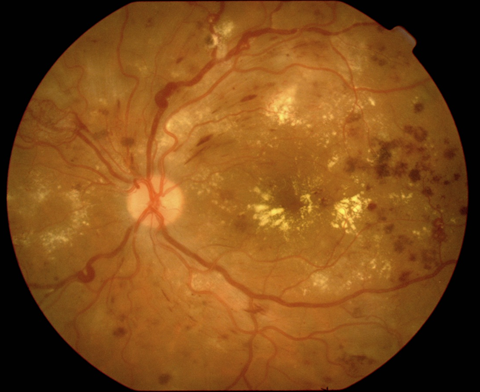
\includegraphics[width=\textwidth]{./figures/ica_retine_maps/G3-P4/g3.png}
		\caption{Original image}	
	\end{subfigure}
	\begin{subfigure}[b]{0.28\textwidth}
		\centering
		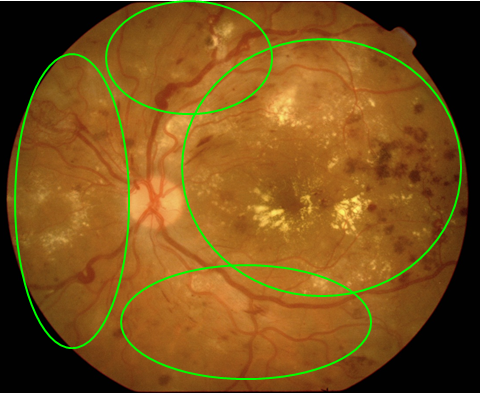
\includegraphics[width=\textwidth]{./figures/ica_retine_maps/G3-P4/metge.png}
		\caption{Real lesion zones}	
	\end{subfigure}
	\hfill 
	\caption{Class 4 image}  
	\label{fig:ica_components_class4_from} 
\end{figure}


\begin{figure}[h!]
	\centering
	\begin{subfigure}[b]{0.32\textwidth}
		\centering
		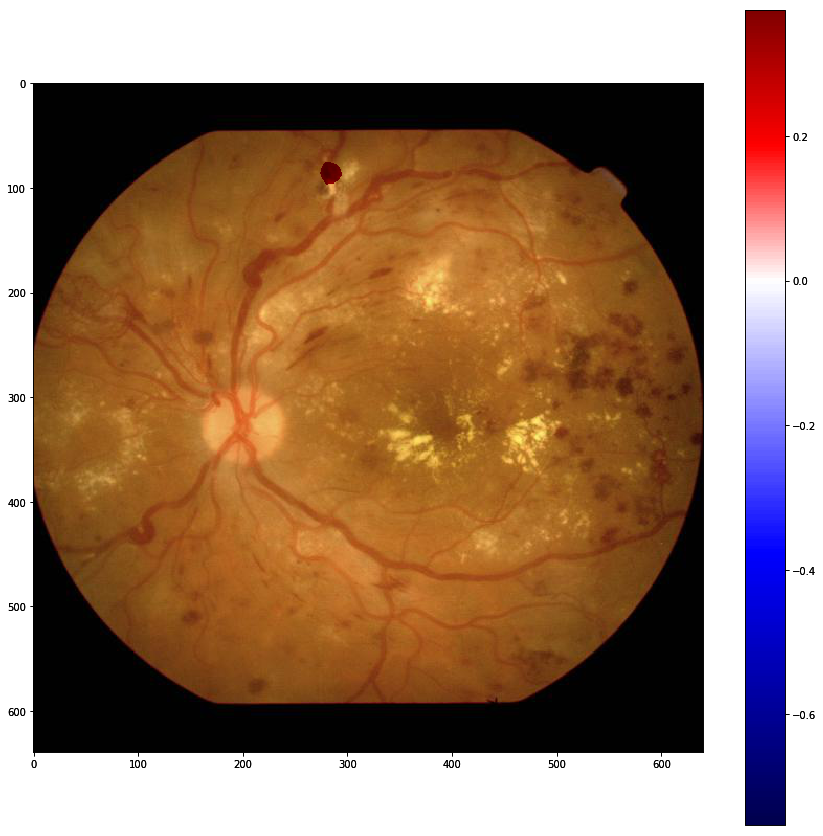
\includegraphics[width=\textwidth]{./figures/ica_retine_maps/G3-P4/m20.png}
		\caption{$ICA_0 < - 3 \sigma$}	
	\end{subfigure}
	\begin{subfigure}[b]{0.32\textwidth}
		\centering
		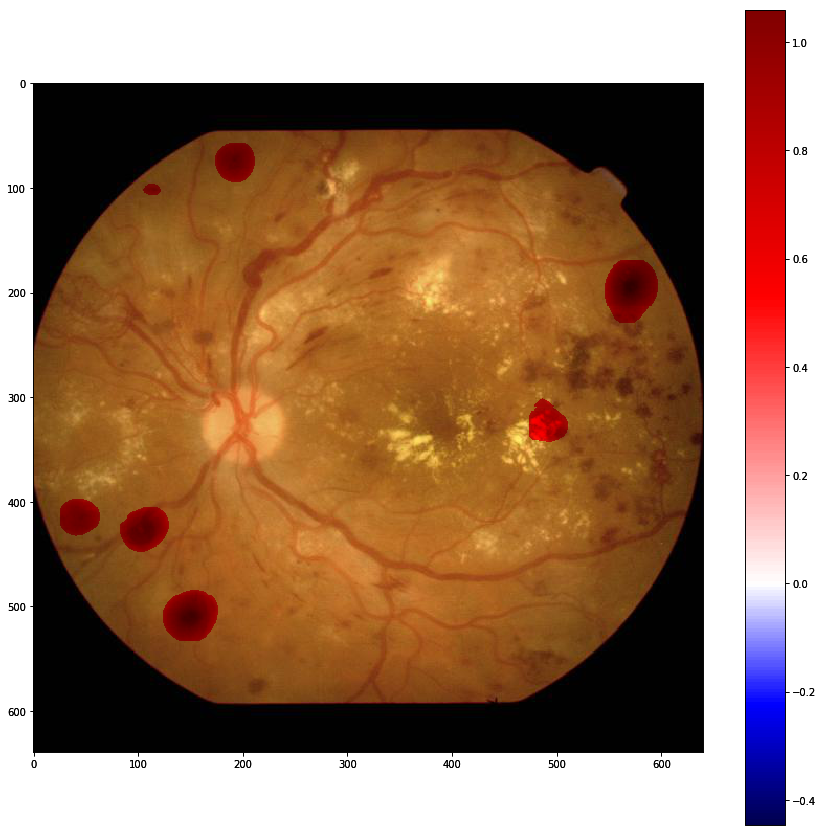
\includegraphics[width=\textwidth]{./figures/ica_retine_maps/G3-P4/m21.png}
		\caption{$ICA_1 < - 3 \sigma$}	
	\end{subfigure}
	\begin{subfigure}[b]{0.32\textwidth}
		\centering
		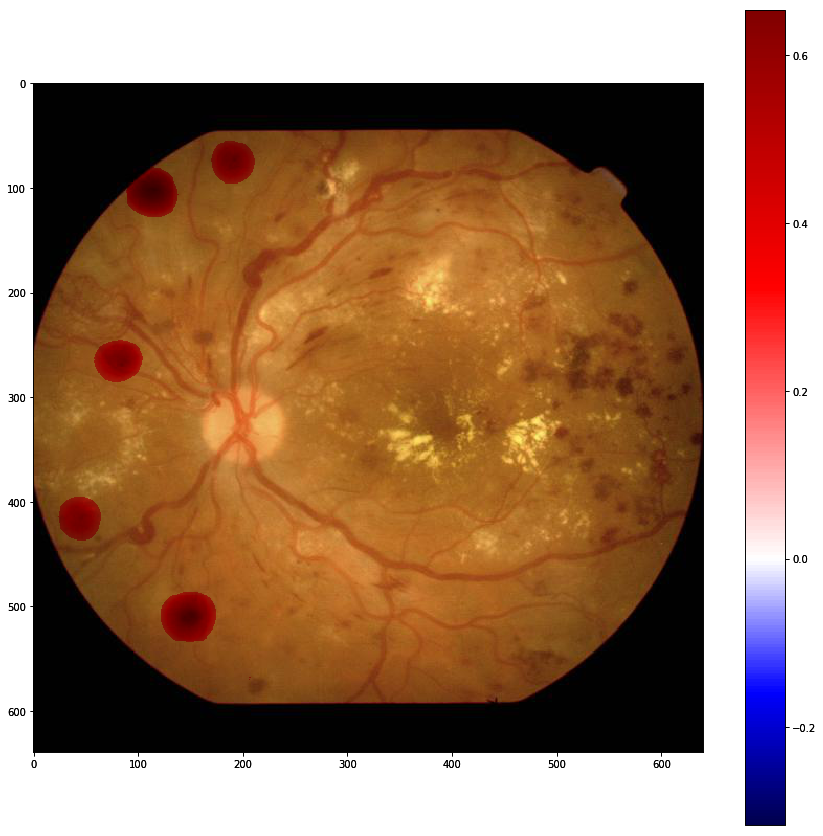
\includegraphics[width=\textwidth]{./figures/ica_retine_maps/G3-P4/m22.png}
		\caption{$ICA_2 < - 3 \sigma$}	
	\end{subfigure}
	\hfill 
	\caption{ICA explanation maps generated using a receptive field of 61x61}  
	\label{fig:ica_components_class4} 
\end{figure}


\added{Figure \ref{ica_components_class4_from} show an example of a proliferative case of DR. We present the results obtained from the model to an expert ophtalmologist in order to validate the results. The expert concludes that all the regions identified by $ICA_1$ and $ICA_2$ correspond to real lesions. In the case of $ICA_0$, the small lesion detected in the top of the image is also a real lesion. In this case, the nature of the lesion is different from the other but it is also caused by the diabetic retinopathy disease.}

\section{Discussion}\label{sec:discussion}


\added{With the compression technique presented in this paper and the use of a visualization technique, we can generate explanation maps as the ones shown in the previous section. This kind of maps provide a very valuable information to the ophthalmologists when they need to make a diagnosis of the degree of development of the DR disease. Some of the eye lesions are so small and the color is so similar to the eye background that its location and identification is really difficult for the person. 
However, if images are preprocessed with this method and some regions are marked, the person can pay 
attention to these parts of the image in order to verify if there are some lesions there.}

The pixels with higher negative signals in the three components will give us the points that are contributing the most to the signaling of a possible presence of the disease. Backpropagating the scores of each one of these negative components will give evidences that help to the distinction of the signs of the final diagnostic given by the deep learning model.

An important point of the results obtained is that the QWK scores obtained with the initial model and the compressed one are really close. This shows that there is not a difference in the separation capability between the t-SNE map of the original features and the map of the ICA 3 dimensional compressed feature map. For such $1.25\%$ difference in the classification performance index ($\kappa_{orig} = 0.800$ vs $\kappa_{ICA} = 0.790$), we can conclude that the independent component analysis has been able to find a adequate compressed expression of the information encoded in the network in a much reduced set of vectors.
\added{Thus, the method has been able to find independent vectors that are able to represent the classes of diabetic retinopathy from the information extracted from a deep learning model.}

\added{We compare the performance of ICA unsupervised compression with other linear compression techniques. Using 3 PCA components, that explain 91\% of the variance a $\kappa_{PCA} = 0.695$ is obtained. Far from the obtained ICA performance.}

\added{It is worth to note that the visualization process of the information coming from these independent vectors in the original image can be done at different levels of generality, depending on the layer of the network.} Hidden layer maps of figures \ref{fig:ica_components_class1}, \ref{fig:ica_components_class2} and \ref{fig:ica_components_class4} are useful when a general map of the lesion locations is enough. Input-space pixel scores are the most suitable when pixel detail is required for detecting the individual lesions causing the disease.

\added{The utility of such maps has been positively corroborated by some ophthalmologists, experts in DR diagnosis. Moreover, they have validated that score maps have an almost perfect match with real lesions having a very low rate of false positives and false negatives. It seems that, $ICA_0$ include sometimes some statistical regularities not directly related with relevant lesions. From such interpretation we conclude that ICA acts as a filter separating lesion information present in images from blink artifacts, noise and other statistical regularities present in images. Such artifacts are found mainly in $ICA_0$.}

\section{Conclusions}\label{sec:conclusions}

In this paper, we studied some of the feature space properties of a already trained diabetic retinopathy deep learning classifier of 17 layers. We saw how, even being a small network, the redundancy of the feature space is very high. We hypothesized that if the network is able to achieve human-level classifications, in some way, it has been able to identify the important statistical regularities present in the image that are important for the classification. As last layer is a linear classifier, such properties has to be disentangled, ie. expressed in a linear way in such last layer. We applied a independent component analysis over such last layer with the method explained in the paper in order to find the optimal number of components that maximize the classification capabilities of such compressed version of the features. We experimentally proved that reducing to only 3 components is possible to achieve almost $99\%$ of the evaluation metric. Such value experimentally prove that the ICA compression has been able to extract all the important elements required for the classification. With such elements, we applied a visualization technique for identifying the elements in the image of each one of the components, using a pixel-wise derived visualization technique. We are able to generate three maps for every image each one identifying independent statistical regularities important for the classification.

\added{Being able to find independent components is important to explore the possibility of using a machine learning method that builds a decision model that uses these vectors together with other patient's data to make a better diagnosis of the patient's risk of developing Diabetic Retinopathy. In fact, we have
started to build such system using fuzzy random forests with information coming from the Electronic Health Record of diabetic patients \cite{saleh2017integration, saleh2018learning}. However, up to now, it is not possible to include the vectors obtained from the images because we do not have a the eye fundus images of the patients of this database. A hospital in our region is now involved on collecting the appropriate data to make this study possible.}

Finally, the method presented in this paper allows not only the classification of retinographies but also the identification and localization in the image of the mathematicaly independent features found by the classifier. The presented ICA score model is of general applicability and can be easily adapted for the usage in other image classification tasks thus, as future work we plan to test it in other types medical images (eg. cancer detection in mammograms).


\section*{Acknowledgements}

This work is supported by the URV grants 2018PFR-URV-B2-61 and 2017PFR-URV-B2-60, and the Spanish research projects PI18/00169 and PI15/01150 (Instituto de Salud Carlos III and Fondos FEDER). The authors would like to thank to Kaggle and EyePACS for providing the data used in this paper.

\section*{References}
\bibliographystyle{unsrt}
\bibliography{retinopathy}

\end{document}
